\documentclass{standalone}
\usepackage{tikz}
\usepackage{ctex,mhchem}
\setCJKmainfont{Noto Serif CJK SC}
\usepackage{mhchem,siunitx}
\begin{document}
\small
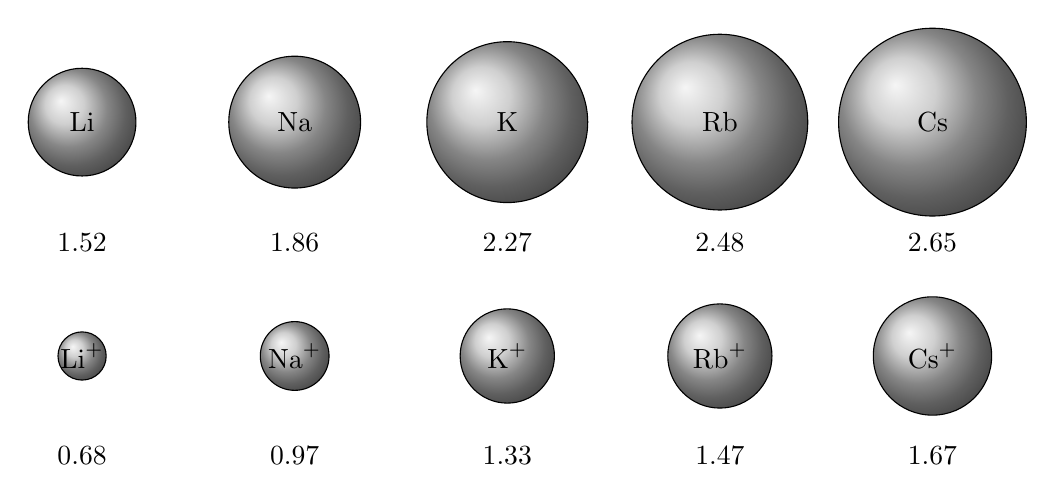
\begin{tikzpicture}[>=stealth,scale=0.9]
  \foreach \x/\r/\R/\a in 
  {
     0/1.52/0.68/Li,
     3/1.86/0.97/Na,
     6/2.27/1.33/K,
     9/2.48/1.47/Rb,
    12/2.65/1.67/Cs%
  }
  {
    \draw[ball color= lightgray] (\x,1.7)circle(0.5*\r)node{\ce{\a}};
    \node at (\x,0){$\r$};
    \draw[ball color= lightgray] (\x,-1.6)circle(0.5*\R)node{\ce{{\a}^+}};
    \node at (\x,-3){$\R$};
  }
\end{tikzpicture}
\end{document}